\let\negmedspace\undefined
\let\negthickspace\undefined
\documentclass[journal,12pt,onecolumn]{IEEEtran}
\usepackage{cite}
\usepackage{amsmath,amssymb,amsfonts,amsthm}
\usepackage{algorithmic}
\usepackage{graphicx}
\usepackage{textcomp}
\usepackage{xcolor}
\usepackage{txfonts}
\usepackage{listings}
\usepackage{enumitem}
\usepackage{mathtools}
\usepackage{gensymb}
\usepackage[breaklinks=true]{hyperref}
\usepackage{tkz-euclide} % loads  TikZ and tkz-base
\usepackage{listings}
\usepackage{amsmath}
\usetikzlibrary{calc, shapes.geometric, angles, quotes}
\usetikzlibrary{patterns}


\newtheorem{theorem}{Theorem}[section]
\newtheorem{problem}{Problem}
\newtheorem{proposition}{Proposition}[section]
\newtheorem{lemma}{Lemma}[section]
\newtheorem{corollary}[theorem]{Corollary}
\newtheorem{example}{Example}[section]
\newtheorem{definition}[problem]{Definition}
%\newtheorem{thm}{Theorem}[section] 
%\newtheorem{defn}[thm]{Definition}
%\newtheorem{algorithm}{Algorithm}[section]
%\newtheorem{cor}{Corollary}
\newcommand{\BEQA}{\begin{eqnarray}}
\newcommand{\EEQA}{\end{eqnarray}}
\newcommand{\define}{\stackrel{\triangle}{=}}
\theoremstyle{remark}
\newtheorem{rem}{Remark}
%\bibliographystyle{ieeetr}
\begin{document}
%
\providecommand{\pr}[1]{\ensuremath{\Pr\left(#1\right)}}
\providecommand{\prt}[2]{\ensuremath{p_{#1}^{\left(#2\right)} }}        % own macro for this question
\providecommand{\qfunc}[1]{\ensuremath{Q\left(#1\right)}}
\providecommand{\sbrak}[1]{\ensuremath{{}\left[#1\right]}}
\providecommand{\lsbrak}[1]{\ensuremath{{}\left[#1\right.}}
\providecommand{\rsbrak}[1]{\ensuremath{{}\left.#1\right]}}
\providecommand{\brak}[1]{\ensuremath{\left(#1\right)}}
\providecommand{\lbrak}[1]{\ensuremath{\left(#1\right.}}
\providecommand{\rbrak}[1]{\ensuremath{\left.#1\right)}}
\providecommand{\cbrak}[1]{\ensuremath{\left\{#1\right\}}}
\providecommand{\lcbrak}[1]{\ensuremath{\left\{#1\right.}}
\providecommand{\rcbrak}[1]{\ensuremath{\left.#1\right\}}}
\newcommand{\sgn}{\mathop{\mathrm{sgn}}}
\providecommand{\abs}[1]{\left\vert#1\right\vert}
\providecommand{\res}[1]{\Res\displaylimits_{#1}} 
\providecommand{\norm}[1]{\left\lVert#1\right\rVert}
%\providecommand{\norm}[1]{\lVert#1\rVert}
\providecommand{\mtx}[1]{\mathbf{#1}}
\providecommand{\mean}[1]{E\left[ #1 \right]}
\providecommand{\cond}[2]{#1\middle|#2}
\providecommand{\fourier}{\overset{\mathcal{F}}{ \rightleftharpoons}}
\newenvironment{amatrix}[1]{%
  \left(\begin{array}{@{}*{#1}{c}|c@{}}
}{%
  \end{array}\right)
}
%\providecommand{\hilbert}{\overset{\mathcal{H}}{ \rightleftharpoons}}
%\providecommand{\system}{\overset{\mathcal{H}}{ \longleftrightarrow}}
	%\newcommand{\solution}[2]{\textbf{Solution:}{#1}}
\newcommand{\solution}{\noindent \textbf{Solution: }}
\newcommand{\cosec}{\,\text{cosec}\,}
\providecommand{\dec}[2]{\ensuremath{\overset{#1}{\underset{#2}{\gtrless}}}}
\newcommand{\myvec}[1]{\ensuremath{\begin{pmatrix}#1\end{pmatrix}}}
\newcommand{\mydet}[1]{\ensuremath{\begin{vmatrix}#1\end{vmatrix}}}
\newcommand{\myaugvec}[2]{\ensuremath{\begin{amatrix}{#1}#2\end{amatrix}}}
\providecommand{\rank}{\text{rank}}
\providecommand{\pr}[1]{\ensuremath{\Pr\left(#1\right)}}
\providecommand{\qfunc}[1]{\ensuremath{Q\left(#1\right)}}
	\newcommand*{\permcomb}[4][0mu]{{{}^{#3}\mkern#1#2_{#4}}}
\newcommand*{\perm}[1][-3mu]{\permcomb[#1]{P}}
\newcommand*{\comb}[1][-1mu]{\permcomb[#1]{C}}
\providecommand{\qfunc}[1]{\ensuremath{Q\left(#1\right)}}
\providecommand{\gauss}[2]{\mathcal{N}\ensuremath{\left(#1,#2\right)}}
\providecommand{\diff}[2]{\ensuremath{\frac{d{#1}}{d{#2}}}}
\providecommand{\myceil}[1]{\left \lceil #1 \right \rceil }
\newcommand\figref{Fig.~\ref}
\newcommand\tabref{Table~\ref}
\newcommand{\sinc}{\,\text{sinc}\,}
\newcommand{\rect}{\,\text{rect}\,}
%%
%	%\newcommand{\solution}[2]{\textbf{Solution:}{#1}}
%\newcommand{\solution}{\noindent \textbf{Solution: }}
%\newcommand{\cosec}{\,\text{cosec}\,}
%\numberwithin{equation}{section}
%\numberwithin{equation}{subsection}
%\numberwithin{problem}{section}
%\numberwithin{definition}{section}
%\makeatletter
%\@addtoreset{figure}{problem}
%\makeatother

%\let\StandardTheFigure\thefigure
\let\vec\mathbf

\bibliographystyle{IEEEtran}


\vspace{3cm}



\bigskip

\renewcommand{\thefigure}{\theenumi}
\renewcommand{\thetable}{\theenumi}
%\renewcommand{\theequation}{\theenumi}
\section{Vectors}
\begin{enumerate}
\item The distance of the point $\brak{-3,4}$ from the $x-axis$ is
\begin{enumerate}
\item $3$\\
\item $-3$\\
\item $4$\\
\item $5$\\
\end{enumerate}
%vectors
\item In Figure $1$, $P\brak{5,-3}$ and $Q\brak{3,y}$ are the points of trisection of the line segment joining $A\brak{7,-2}$ and $B\brak{1,-5}$.Then $y$ is equals
\begin{figure} [h]
\centering
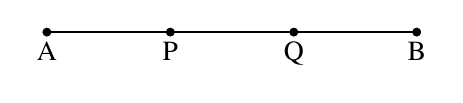
\begin{tikzpicture}[scale=0.7]
\draw[thick] 
    (-5.37, 4.92) --  % A
    (-3.13, 4.92) --  % P
    (-0.89, 4.92) --  % Q
    (1.34, 4.92) -- cycle;  % B
\node at (-5.37, 4.92) [below] {A};
\node at (-3.13, 4.92) [below] {P};
\node at (-0.89, 4.92) [below] {Q};
\node at (1.34, 4.92) [below] {B};
\filldraw 
    (-5.37, 4.92) circle (2pt)  % A
    (-3.13, 4.92) circle (2pt)  % P
    (-0.89, 4.92) circle (2pt)  % Q
    (1.34, 4.92) circle (2pt);  % B

\end{tikzpicture}
\end{figure}
\begin{center}
$\text{Figure } 1$
\end{center}
\begin{enumerate}
\item $2$\\
\item $4$\\
\item $-4$\\
\item $\dfrac{-5}{2}$\\
\end{enumerate}
\item The coordinates of the point $P$ dividing the line segment joining the points $A\brak{1,3}$ and $B\brak{4,6}$, in the ratio $2:1$ are:
\begin{enumerate}
\item $\brak{2,4}$\\
\item $\brak{3,5}$\\
\item $\brak{4,2}$\\
\item $\brak{5,3}$\\
\end{enumerate}
%circles
\item If the coordinates of one end of a diameter of a circle are $\brak{2,3}$ and the coordinates of its centre are $\brak{-2,5}$, then the coordinates of the other end of the diameter are:
\begin{enumerate}
\item $\brak{-6,7}$\\
\item $\brak{6,-7}$\\
\item $\brak{6,7}$\\
\item $\brak{-6,-7}$\\
\end{enumerate}
\item The area of a triangle whose vertices are $\brak{5,0}$, $\brak{8,0}$ and $\brak{8,4}$ $\brak{\text{in sq. units}}$ is
\begin{enumerate}
\item $20$\\
\item $12$\\
\item $6$\\
\item $16$\\
\end{enumerate}

\item If $A\brak{1,3}$, $B\brak{-1,2}$, $C\brak{2,5}$ and $D\brak{x,4}$ are the vertices of a parallelogram $ABCD$, then the value of $x$ is
\begin{enumerate}
\item $3$\\
\item $4$\\
\item $0$\\
\item $\dfrac{3}{2}$\\
\end{enumerate}
%vectors
\item Find the value of $k$, if the point $P\brak{2,4}$ is equidistant from the points $A\brak{5,k}$ and $B\brak{k,7}$.\\
%vectors
\item Find the coordinates of a point $P$, which lies on the line segment joining the points $A\brak{-2,2}$ and $B\brak{2,-4}$ such that $AP = \frac{3}{7} AB$.\\
%vectors

%vectors
\item If a point $A\brak{0,2}$ is equidistant from the points $B\brak{3,p}$ and $C\brak{p,5}$, then find the value of $p$.\\
%vectors
\item A point $P$ divides the line segment joining the points $A\brak{3,-5}$ and $B\brak{-4,8}$ such that $\dfrac{AP}{PB} = \dfrac{K}{1}$. If $P$ lies on the line $x + y = 0$, then find the value of $K$.\\
\item Find the ratio in which the line segment joining the points $\brak{1,-3}$ and $\brak{4,5}$ is divided by x-axis.\\
\item Find the ratio in which the y-axis divides the line segment joining the points \brak{5,-6}$ and \brak{-1,-4}$. Also find the coordinates of the point of intersection.\\

\item For what value of $k$, $\brak{ k > 0}$, s the area of the triangle with vertices $\brak{-2,5}$, \brak{k,-4}$, and \brak{2k+1,10}$ equal to $52$ sq. units?\\

\item If the vertices of a triangle are $\brak{1,-3}$, $\brak{4,p}$ and $\brak{-9,7}$ and its area is $15$ sq. units, find the value$\brak{\text{s}}$ of $p$.\\
\item Find the area of quadrilateral $ABCD$ whose vertices are $A\brak{-3,-1}$, $B\brak{-2,-4}$, $C\brak{4,-1}$ and $D\brak{3,4}$.\\

\item If the point $A\brak{x,y}$, $B\brak{3,6}$ and $C\brak{-3,4}$ are collinear, show that $x - 3y + 15 = 0$.\\
\end{enumerate}
\section{Circles}
\begin{enumerate}
\item From a point $Q$, $13 \text{ cm}$ away from the centre of a circle, the length of tangent $PQ$ to the circle is $12 \text{ cm}$. The radius of circle \brak{\text{in $cm$}}
\begin{enumerate}
\item $25$\\
\item $\sqrt{313}$\\
\item $5$\\
\item $1$\\
\end{enumerate}
%circles
\item In Figure $1$, $AP$, $AQ$ and $BC$ are tangents to the circle. If $AB = 5 \text{cm}$, $AC = 6 \text{ cm}$ and $BC = 4 \text{ cm}$, then the length of $AP$ \brak{\text{in $cm$}} is
\begin{figure} [h]
\centering
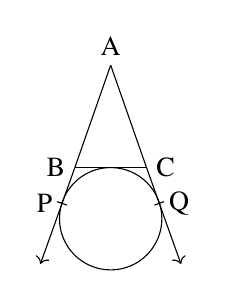
\begin{tikzpicture}[scale=0.65]

% Circle
\draw (0,0) circle (1cm);

% Points
\coordinate (A) at (0,3);
\coordinate (B) at (-0.7, 1);
\coordinate (C) at (0.7, 1);
\coordinate (P) at (-0.95, 0.3);
\coordinate (Q) at (0.95, 0.3);

% Tangents and Lines
\draw (A) -- (B) node[midway, left] {};
\draw (A) -- (C) node[midway, right] {};
\draw (B) -- (C) node[midway, below] {};
\draw (B) -- (P);
\draw (C) -- (Q);

% Arrows
\draw[->] (P) -- ($(B)!2cm!(P)$);
\draw[->] (Q) -- ($(C)!2cm!(Q)$);

% Perpendicular lines
\draw ($(P)!0.1cm!90:(B)$) -- ($(P)!0.1cm!-90:(B)$);
\draw ($(Q)!0.1cm!90:(C)$) -- ($(Q)!0.1cm!-90:(C)$);

% Labeling points
\node at (A) [above] {A};
\node at (B) [left] {B};
\node at (C) [right] {C};
\node at (P) [left] {P};
\node at (Q) [right] {Q};
\end{tikzpicture}
\end{figure}
\begin{center}
$\text{Figure } 1$
\end{center}
\begin{enumerate}
\item $7.5$\\
\item $15$\\
\item $10$\\
\item $9$\\
\end{enumerate}
%circles
\item The circumference of a circle is $22 \text{ cm}$. The area of its quadrant \brak{\text{in $cm^2$}}
\begin{enumerate}
\item $\dfrac{77}{2}$\\
\item $\dfrac{77}{4}$\\
\item $\dfrac{77}{8}$\\
\item $\dfrac{77}{16}$\\
\end{enumerate}
\item In Figure $2$, a right triangle $ABC$, circumscribe a circle of radius $r$. If $AB$ and $BC$ are of lengths $8 \text{ cm}$ and $6 \text{ cm}$ respectively, find the value of $r$.
\begin{figure}[ht]
\centering
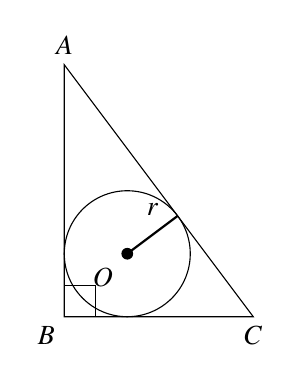
\begin{tikzpicture}[scale=0.4]
    % Triangle ABC
    \coordinate[label=above:$A$] (A) at (0,8);
    \coordinate[label=below left:$B$] (B) at (0,0);
    \coordinate[label=below:$C$] (C) at (6,0);
    \draw (A) -- (B) -- (C) -- cycle;
    
    % Point (18/5, 16/5)
    \coordinate[label=above:$ $] (P) at (3.6,3.2);
    \fill (P) circle (0pt);
    
    % Line and length r
    \draw[thick] (2,2) -- (3.6,3.2);
    \node[label=below left:$O$,circle,fill,inner sep=1.5pt] (O) at (2,2) {};
    \node[label=above:$r$] at (2.8,2.6) {};
    \draw (O) circle (2cm);
    % Right angle at B
    \draw pic["$ $", draw=black, angle radius=0.4cm, angle eccentricity=1.5] {right angle = C--B--A};
\end{tikzpicture}
\end{figure}
\begin{center}
$\text{Figure } 2$
\end{center}
\item In Figure $3$, $PQ$ and $PR$ are tangents to a circle with centre $A$. If $\angle QPA = 27\degree$, then $\angle QAR$ equals
\begin{figure}[ht]
\centering
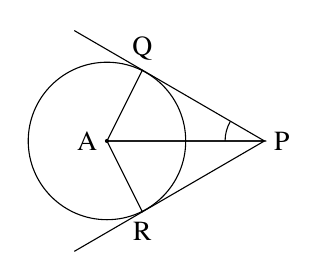
\begin{tikzpicture}[scale=1]
  % Define points
  \coordinate (A) at (0,0);
  \coordinate (Q) at (0.45,0.9); % This point is 60 degrees above the horizontal.
  \coordinate (P) at (2,0);     % Chosen arbitrarily, adjust as needed.
  \coordinate (R) at (0.45,-0.9); % Midpoint of AP
  
  % Draw circle with center A through point Q
  \draw (A) circle (1cm);
  
  % Draw triangle APQ
  \draw (A) -- (P) -- (Q) -- cycle;
  \draw (A) -- (P) -- (R) -- cycle;
  \draw (0.45,0.9) -- (-0.415,1.402);
  \draw (0.45,-0.9) -- (-0.415,-1.402);
  
  % Label points
  \node at (A) [left] {A};
  \node at (P) [right] {P};
  \node at (Q) [above] {Q};
  \node at (R) [below] {R};
  \fill (0,0) circle (0.75pt);

  % Draw the angle arc % Draw the angle with label
  \pic [draw, "$ $", angle eccentricity = 1, angle radius=0.5cm] {angle = Q--P--A};


\end{tikzpicture}
\end{figure}
\begin{center}
$\text{Figure } 3$
\end{center}
\begin{enumerate}
\item $63\degree$\\
\item $153\degree$\\
\item $126\degree$\\
\item $117\degree$\\
\end{enumerate}
\item In Figure $4$, $AB$ and $AC$ are tangents to a circle with centre $O$ and radius $8\text{ cm}$. If $OA = 17\text{ cm}$, then the length of $AC \brak{\text { in cm}}$  is
\begin{figure}[ht]
\centering
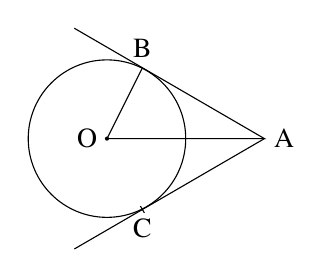
\begin{tikzpicture}[scale=1]
  % Define points
  \coordinate (O) at (0,0);
  \coordinate (B) at (0.45,0.9); % This point is 60 degrees above the horizontal.
  \coordinate (A) at (2,0);     % Chosen arbitrarily, adjust as needed.
  \coordinate (C) at (0.45,-0.9); % Midpoint of AP
  
  % Draw circle with center A through point Q
  \draw (O) circle (1cm);
  
  % Draw triangle APQ
  \draw (O) -- (A) -- (B) -- cycle;
  \draw (A) -- (C);
  \draw (0.45,0.9) -- (-0.415,1.402);
  \draw (0.45,-0.9) -- (-0.415,-1.402);
  \draw ($(C)!0.05cm!90:(A)$) -- ($(C)!0.05cm!-90:(A)$);
  
  % Label points
  \node at (O) [left] {O};
  \node at (A) [right] {A};
  \node at (B) [above] {B};
  \node at (C) [below] {C};
  \fill (0,0) circle (0.75pt);

\end{tikzpicture}
\end{figure}
\begin{center}
$\text{Figure } 4$
\end{center}
\begin{enumerate}
\item $\sqrt {353}$\\
\item $15$\\
\item $9$\\
\item $25$\\
\end{enumerate}
\item In Figure $5$, three sectors of a circle of radius $7\text{ cm}$, making angles of $60\degree$, $80\degree$, $40\degree$ at the centre are shaded. The area of the shaded region $\brak{in\text{ cm}^2}$ is $\brak{\text{Using } \pi = \frac{22}{7}}$
\begin{figure}[ht]
\centering
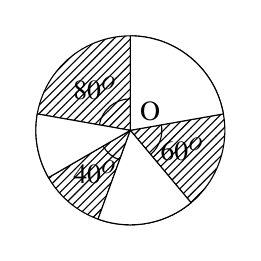
\begin{tikzpicture}[scale = 1.2, rotate=10]
  % Define the radius of the circle
  \def\radius{1cm}
  
  % Draw the circle
  \draw (0,0) circle (1cm);
  
  % Define points for the angles
  \coordinate (O) at (0,0);
  \coordinate (A) at (1,0);
  \coordinate (C) at (80:1);
  \coordinate (D) at (160:1);
  \coordinate (E) at (200:1);
  \coordinate (F) at (240:1);
  \coordinate (B) at (300:1);

  % Draw the angle arc % Draw the angle with label
  \pic [draw, "$60^O$", angle eccentricity=1.75, angle radius=0.4cm] {angle = B--O--A};
  \pic [draw, "$80^O$", angle eccentricity=1.75, angle radius=0.4cm] {angle = C--O--D};
  \pic [draw, "$40^O$", angle eccentricity=1.75, angle radius=0.4cm] {angle = E--O--F};
  
  % Draw the sectors and lines
  \draw (O) -- (A) (O) -- (B) (O) -- (C);
  \draw (O) -- (D) (O) -- (E) (O) -- (F);

  \fill[pattern=north east lines] (0,0) circle (1cm);

  % Draw the quadrants
  \draw[fill=white] (O) -- (A) arc [start angle=0, end angle=80, radius=1] -- cycle;
  \draw[fill=white] (O) -- (D) arc [start angle=160, end angle=200, radius=1] -- cycle;
  \draw[fill=white] (O) -- (F) arc [start angle=240, end angle=300, radius=1] -- cycle;
  
  % Label the center
  \node at (O) [above right] {O};

\end{tikzpicture}
\end{figure}
\begin{center}
$\text{Figure } 5$
\end{center}
\begin{enumerate}
\item $77$\\
\item $154$\\
\item $44$\\
\item $22$\\
\end{enumerate}
\item In Figure $6$, the sides $AB$, $BC$ and $CA$ of a triangle $ABC$, touch a circle at $P$, $Q$ and $R$ respectively. If $PA = 4\text{ cm}$, $BP = 3\text{ cm}$ and $AC = 11\text{ cm}$, then the length of $BC$ \brak{\text{in $cm$}} is
\begin{figure}[ht]
\centering
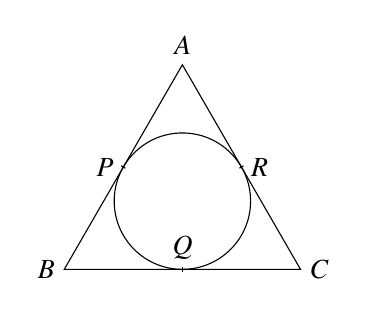
\begin{tikzpicture}[scale=0.3]
  % Define coordinates for the vertices of the triangle
  \coordinate[label=left:$B$] (B) at (0,0);
  \coordinate[label=right:$C$] (C) at (10,0);
  \coordinate[label=above:$A$] (A) at (5,8.6603);

  % Draw the triangle
  \draw (A) -- (B) -- (C) -- cycle;

 % Draw the circle with centre (0.5,0.28868) and radius 0.28868
    \draw (5,2.8868) circle (2.8868);

  % Label the incenter. Adjust the label position as needed
  \coordinate[label=left:$P$] (P) at (2.5,4.33015);
  \coordinate[label=above:$Q$] (Q) at (5,0);
  \coordinate[label=right:$R$] (R) at (7.5,4.33015);
  % Drawing perpendicular lines
  \draw ($(Q)!0.1cm!90:(B)$) -- ($(Q)!0.1cm!-90:(B)$);
  \draw ($(R)!0.1cm!90:(C)$) -- ($(R)!0.1cm!-90:(C)$);
  \draw ($(P)!0.1cm!90:(B)$) -- ($(P)!0.1cm!-90:(B)$);

\end{tikzpicture}
\end{figure}
\begin{center}
$\text{Figure } 6$
\end{center}
\begin{enumerate}
\item $11$\\
\item $10$\\
\item $14$\\
\item $15$\\
\end{enumerate}
%circles
\item In Figure $7$, a circle touches the side $DF$ of $\triangle EDF$ at $H$ and touches $ED$ and $EF$ produced at $K$ and $M$ respectively. If $EK = 9\text{ cm}$, then the perimeter of $\triangle EDF$ \brak{\text{in $cm$}} is
\begin{figure}[ht]
\centering
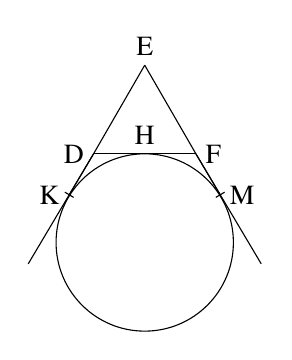
\begin{tikzpicture}[scale=0.65]

% Circle
\draw (1,-1.732) circle (1.73234cm);

% Points
\coordinate (D) at (0,0);
\coordinate (E) at (1, 1.732);
\coordinate (F) at (2, 0);
\coordinate (H) at (1, 0);
\coordinate (K) at (-0.475, -0.8);
\coordinate (M) at (2.475, -0.8);

% Tangents and Lines
\draw (D) -- (E) node[midway, left] {};
\draw (E) -- (F) node[midway, right] {};
\draw (F) -- (D) node[midway, below] {};
\draw (D) -- (K);
\draw (F) -- (M);

% Arrows
\draw[-] (D) -- ($(D)!2.5cm!(K)$);
\draw[-] (F) -- ($(F)!2.5cm!(M)$);

% Perpendicular lines
\draw ($(K)!0.1cm!90:(D)$) -- ($(K)!0.1cm!-90:(D)$);
\draw ($(M)!0.1cm!90:(F)$) -- ($(M)!0.1cm!-90:(F)$);

% Labeling points
\node at (E) [above] {E};
\node at (D) [left] {D};
\node at (F) [right] {F};
\node at (H) [above] {H};
\node at (K) [left] {K};
\node at (M) [right] {M};

\end{tikzpicture}
\end{figure}
\begin{center}
$\text{Figure } 7$
\end{center}
\begin{enumerate}
\item $18$\\
\item $13.5$\\
\item $12$\\
\item $9$\\
\end{enumerate}
%circles
\item If the area of a circle is equal to sum of the areas of two circles of diameters $10 \text{ cm}$ and $24 \text{ cm}$, then the diameter of the larger circle \brak{\text{in $cm$}} is
\begin{enumerate}
\item $34$\\
\item $26$\\
\item $17$\\
\item $14$\\
\end{enumerate}
%Circles
\item Prove that the tangents drawn at the ends of a diameter of a circle are parallel.\\
%circles
\item In Figure $8$, $ABCD$ is a square of side $4 \text{ cm}$. A quadrant of a circle of radius $1 \text{ cm}$ is drawn at each vertex of the square and a circle of diameter $2 \text{ cm}$ is also drawn. Find the area of the shaded region. $\brak{\text{Use } \pi = 3.14}$
\begin{figure}[ht]
\centering
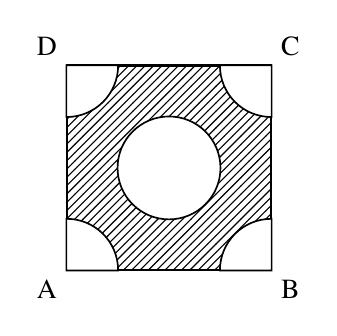
\begin{tikzpicture}[scale=0.65]
    % Draw the square
    \draw[thick] (0,0) rectangle (4,4);
    
    % Draw the circle
    \draw[thick,fill=white] (2,2) circle [radius=1];
    
    % Draw the quadrants
    \draw[thick,fill=white] (0,0) -- (1,0) arc [start angle=0, end angle=90, radius=1] -- cycle;
    \draw[thick,fill=white] (4,0) -- (3,0) arc [start angle=180, end angle=90, radius=1] -- cycle;
    \draw[thick,fill=white] (4,4) -- (3,4) arc [start angle=180, end angle=270, radius=1] -- cycle;
    \draw[thick,fill=white] (0,4) -- (1,4) arc [start angle=360, end angle=270, radius=1] -- cycle;
    
    % Add the hatching pattern with controlled density
    \path[pattern=north east lines, pattern color=black] (0,0) rectangle (4,4);
    
    % Exclude the circle and quadrants from the hatching by overlaying with white fill
    \draw[fill=white] (2,2) circle [radius=1];
    \draw[fill=white] (0,0) -- (1,0) arc [start angle=0, end angle=90, radius=1] -- cycle;
    \draw[fill=white] (4,0) -- (3,0) arc [start angle=180, end angle=90, radius=1] -- cycle;
    \draw[fill=white] (4,4) -- (3,4) arc [start angle=180, end angle=270, radius=1] -- cycle;
    \draw[fill=white] (0,4) -- (1,4) arc [start angle=360, end angle=270, radius=1] -- cycle;
    \node at (0,0) [below left] {A};
    \node at (4,0) [below right] {B};
    \node at (4,4) [above right] {C};
    \node at (0,4) [above left] {D};
\end{tikzpicture}
\end{figure}
\begin{center}
$\text{Figure } 8$
\end{center}
%Circles
\item From a rectangular sheet of paper $ABCD$ with $AB = 40 \text{ cm}$ and $AD = 28 \text{ cm}$, a semi-circular portion with $BC$ as diameter is cut off. Find the area of the remaining paper. $\brak{\text{Use } \pi = \frac{22}{7}}$\\
%Circles
\item In Figure $9$, a circle is inscribed in a triangle $PQR$ with $PQ = 10 \text{ cm}$, $QR = 8 \text{ cm}$ and $PR = 12 \text{ cm}$. Find the lengths of $QM$, $RN$ and $PL$.
\begin{figure}[ht]
\centering
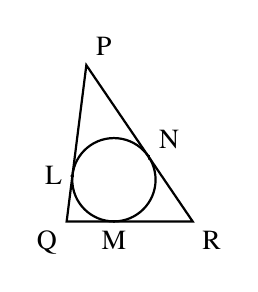
\begin{tikzpicture}[scale=0.2]

% Define points
\coordinate (P) at (1.25,9.92);
\coordinate (Q) at (0,0);
\coordinate (R) at (8,0);
\coordinate (N) at (5.25,4);
\coordinate (L) at (0.33,2.9);
\coordinate (M) at (3,0);

% Draw triangle and lines
\draw[thick] (P) -- (Q) -- (R) -- cycle;
\draw[thick] (5.25,4) -- ++(0,-0.08) -- ++(0,0.3); % Perpendicular line at N
\draw[thick] (0.33,2.9) -- ++(-0.08,0) -- ++(0.2,0); % Horizontal line at (0.33,2.9)
\draw[thick] (3,0) -- ++(0,-0.08) -- ++(0,0.2); % Vertical line at M

% Draw incircle
\draw[thick] (3,2.64575) circle (2.64575cm);

% Labels
\node[above right] at (P) {P};
\node[below left] at (Q) {Q};
\node[below right] at (R) {R};
\node[below] at (M) {M};
\node[left] at (L) {L};
\node[above right] at (N) {N};

\end{tikzpicture}
\end{figure}
\begin{center}
$\text{Figure } 9$
\end{center}
%Circles
\item In Figure $10$, $O$ is the centre of the circle with $AC = 24 \text{ cm}$, $AB = 7 \text{ cm}$ and $\angle BOD = 90\degree$. Find the area of shaded region.$\brak{\text{Use } \pi = 3.14}$
\begin{figure}[ht]
\centering
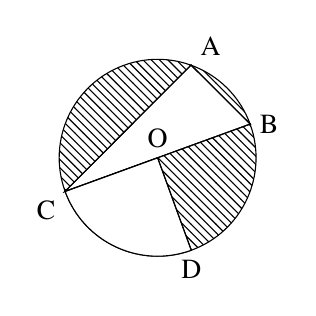
\begin{tikzpicture}[rotate=20, scale=0.1]

% Circle with BC as diameter (for reference in clipping paths)
\coordinate (B) at (12.5,0);
\coordinate (C) at (-12.5,0);
\coordinate (A) at (8,9.6);
\coordinate (O) at (0,0);
\coordinate (D) at (0,-12.5);
\path (B) -- (C) coordinate[midway] (BCmid);

% Hatching the regions excluding quadrant COD and triangle ABC
\path[pattern = north west lines, pattern color=black] (0,0) circle (12.5cm);

% Original circle
\draw (0,0) circle (12.5cm);

% Exclude the circle and quadrants from the hatching by overlaying with white fill
    \draw[fill=white] (B) -- (A) -- (C) -- cycle;
    \draw[fill=white] (0,0) -- (-12.5,0) arc [start angle=180, end angle=270, radius=12.5] -- cycle;

% Labels
\node[above right] at (8,9.6) {A};
\node[right] at (12.5,0) {B};
\node[below left] at (-12.5,0) {C};
\node[above] at (0,0) {O};
\node[below] at (0,-12.5) {D};
% Triangle ABC
\draw [black] (B) -- (A) -- (C) -- cycle;

% Line OD
\draw [black] (O) -- (D);

\end{tikzpicture}
\end{figure}
\begin{center}
$\text{Figure } 10$
\end{center}
\item In Figure $11$, find the area of shaded region, if $ABCD$ is a square of side $14 \text{ cm}$ and $APD$ and $BPC$ are semicircles.
\begin{figure}[ht]
\centering
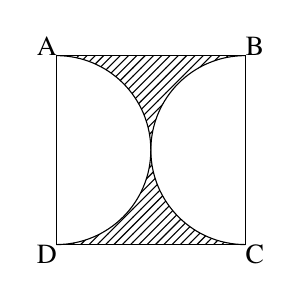
\begin{tikzpicture}[scale=0.6]
  % Draw square
  \draw (0,0) rectangle (4,4);
  
  % Label corners of the square
  \node at (-0.2,-0.2) {D};
  \node at (4.2,-0.2) {C};
  \node at (4.2,4.2) {B};
  \node at (-0.2,4.2) {A};
  
  % Draw and fill the area between the arcs
  \begin{scope}
    \clip (0,4) arc[start angle=90, end angle=-90, radius=2] -- 
          (4,0) arc[start angle=-90, end angle=-270, radius=2];
    \fill[pattern=north east lines] (0,0) rectangle (4,4);
  \end{scope}
  
  % Draw arcs again on top of the fill to make them visible
  \draw (0,4) arc[start angle=90, end angle=-90, radius=2];
  \draw (4,0) arc[start angle=-90, end angle=-270, radius=2];

\end{tikzpicture}
\end{figure}
\begin{center}
$\text{Figure } 11$
\end{center}
%circles
\item Prove that the length of tangents drawn from an external point to a circle are equal.\\

%circles
\item Tangents $PA$ and $PB$ are drawn from an external point $P$ to two concentric circles with centre $O$ and radii $8 \text{ cm}$ and $5 \text{ cm}$ respectively, as shown in Figure $12$. If $AP = 15\text{ cm}$, then find the length of $BP$.
\begin{figure}[ht]
\centering
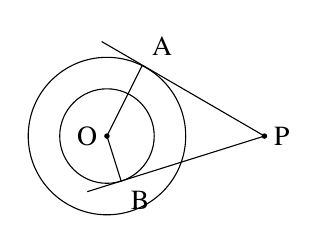
\begin{tikzpicture}[scale=1]
  % Draw the large circle
  \draw (0,0) circle (1cm);
  
  % Draw the middle circle
  \draw (0,0) circle (0.6cm);
  
  % Label the center
  \fill (0,0) circle (1pt) node[left] {O};
  
  % Draw the point P and line OP
  \fill (2,0) circle (1pt) node[right] {P};
  
  
  % Draw and label the tangent line
  \draw (2,0) -- (0.45,0.9) node[above right] {A};
  \draw (2,0) -- (0.18,-0.57148) node[below right] {B};
  
  % Optional: Add arrows to the line to indicate it extends indefinitely
  \draw (0.45,0.9) -- (-0.067,1.2);
  \draw (0.18,-0.57148) -- (-0.25,-0.7065);
  \draw (0,0) -- (0.45,0.9);
  \draw (0,0) -- (0.18,-0.57148);
  
\end{tikzpicture}
\end{figure}
\begin{center}
$\text{Figure } 12$
\end{center}

%circles
\item In Figure $13$, an isosceles triangle $ABC$, with $AB = AC$, circumscribe a circle. Prove that the point of contact $P$ bisects the base $BC$.
\begin{figure}[ht]
\centering
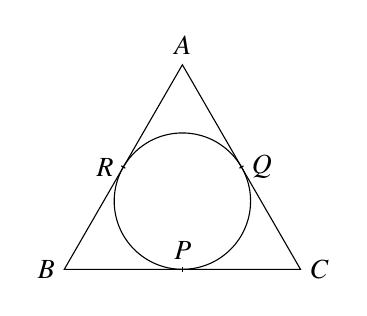
\begin{tikzpicture}[scale=0.3]
  % Define coordinates for the vertices of the triangle
  \coordinate[label=left:$B$] (B) at (0,0);
  \coordinate[label=right:$C$] (C) at (10,0);
  \coordinate[label=above:$A$] (A) at (5,8.6603);

  % Draw the triangle
  \draw (A) -- (B) -- (C) -- cycle;

 % Draw the circle with centre (0.5,0.28868) and radius 0.28868
    \draw (5,2.8868) circle (2.8868);

  % Label the incenter. Adjust the label position as needed
  \coordinate[label=left:$R$] (R) at (2.5,4.33015);
  \coordinate[label=above:$P$] (P) at (5,0);
  \coordinate[label=right:$Q$] (Q) at (7.5,4.33015);
  
  % Drawing perpendicular lines
  \draw ($(P)!0.1cm!90:(B)$) -- ($(P)!0.1cm!-90:(B)$);
  \draw ($(R)!0.1cm!90:(B)$) -- ($(R)!0.1cm!-90:(B)$);
  \draw ($(Q)!0.1cm!90:(C)$) -- ($(Q)!0.1cm!-90:(C)$);

\end{tikzpicture}
\end{figure}
\begin{center}
$\text{Figure } 13$
\end{center}
%circles
\item In Figure $14$, the chord $AB$ of the larger of the two concentric circles, with centre $O$, touches the smaller circle at $C$. Prove that $AC = CB$.
\begin{figure}[ht]
\centering
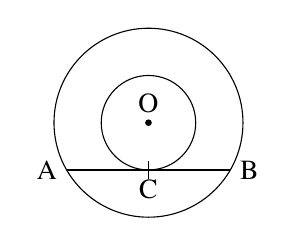
\begin{tikzpicture}[scale=1.2]
  \draw (0,0) circle (1cm);
  
  % Draw the middle circle
  \draw (0,0) circle (0.5cm);
  
  % Label the center
  \fill (0,0) circle (1pt) node[above] {O};
  
  % Draw the points P, A, B, and lines OP, AC, BC
  \coordinate[label=below:C] (C) at (0,-0.5);
  \coordinate[label=left:A] (A) at (-0.866,-0.5);
  \coordinate[label=right:B] (B) at (0.866,-0.5);
  
  % Draw and label the tangent line
  \draw (-0.866,-0.5) -- (0.866,-0.5);
  \draw ($(C)!0.1cm!90:(A)$) -- ($(C)!0.1cm!-90:(A)$);
\end{tikzpicture}
\end{figure}
\begin{center}
$\text{Figure } 14$
\end{center}
%circles
\item In Figure $15$, $OABC$ is a square of side $7 \text{ cm}$. If $OAPC$ is a quadrant of a circle with centre $O$, then find the area of the shaded region. $\brak{\text{Use } \pi = 3.14}$\\
\\
\begin{figure}[ht]
\centering
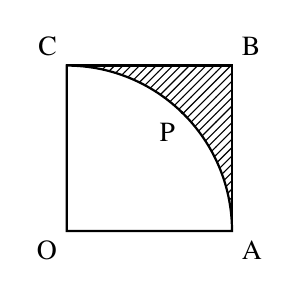
\begin{tikzpicture}[scale=0.3]
    % Draw the square
    \draw[thick] (0,0) rectangle (7,7);
    
    % Add the hatching pattern with controlled density
    \path[pattern=north east lines, pattern color=black] (0,0) rectangle (7,7);
    
    % Draw the quadrants
    \draw[thick,fill=white] (0,0) -- (7,0) arc [start angle=0, end angle=90, radius=7] -- cycle;

    % Label the vertices
    \node at (0,0) [below left] {O};
    \node at (7,0) [below right] {A};
    \node at (7,7) [above right] {B};
    \node at (0,7) [above left] {C};
    \node at (5,5) [below left] {P};
    \fill (4.9,5) circle (2pt);

\end{tikzpicture}
\end{figure}
\begin{center}
$\text{Figure } 15$
\end{center}

\item Prove that the parallelogram circumscribing a circle is rhombus.\\
%circles
\item Prove that opposite sides of a quadrilateral circumscribing a circle subtend supplementary angles at the centre of the circle.\\
%circles
\item In Figure $16$, $PQ$ and $AB$ are respectively the arcs of two concentric circles of radii $7\text{ cm}$ and $3.5\text{ cm}$ and centre $O$. If $\angle POQ = 30\degree$, then find the area of the shaded region. $\brak{\text{Use } \pi = \frac{22}{7}}$
\begin{figure}[ht]
\centering
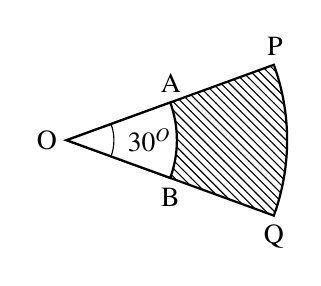
\begin{tikzpicture}[rotate = -20, scale = 0.4]

   \coordinate (O) at (0,0);
   \coordinate (A) at (2.7,2.25);
   \coordinate (B) at (3.5,0);
   \coordinate (P) at (5.4,4.5);
   \coordinate (Q) at (7,0);

    % Draw the quadrants
    \draw[thick] (0,0) -- (7,0) arc [start angle=0, end angle=40, radius=7] -- cycle;
    
    % Add the hatching pattern with controlled density
    \path[pattern=north west lines, pattern color=black] (0,0) -- (7,0) arc [start angle=0, end angle=40, radius=7] -- cycle;

    \draw[thick,fill=white] (0,0) -- (3.5,0) arc [start angle=0, end angle=40, radius=3.5] -- cycle;

    % Label the vertices
    \node at (0,0) [left] {O};
    \node at (2.7,2.25) [above] {A};
    \node at (3.5,0) [below] {B};
    \node at (7,0) [below] {Q};
    \node at (5.4,4.5) [above] {P};

    % Draw the angle arc % Draw the angle with label
  \pic [draw, "$30^O$", angle eccentricity=1.75, angle radius=0.6cm] {angle = Q--O--P};

\end{tikzpicture}
\end{figure}
\begin{center}
$\text{Figure } 16$
\end{center}
\item Prove that the tangent at any point of a circle is perpendicular to the radius through the point of contact.\\

\item A quadrilateral $ABCD$ is drawn to circumscribe a circle. Prove that $AB + CD = AD + BC$.\\

\item The incircle of an isosceles triangle $ABC$, with $AB = AC$, touches the sides $AB$, $BC$ and $CA$ at $D$, $E$ and $F$ respectively. Prove that $E$ bisects $BC$.\\

\item Prove that in two concentric circles. the chord of the larger circle, which touches the smaller circle, is bisected at the point of contact.\\

\item In Figure $17$, the shape of the top of the table is that of a sector of a circle with centre $O$ and $\angle OAB = 90\degree$. If $AO = OB = 42\text{ cm}$, then find the perimeter of the top of the table.
\begin{figure}[ht]
\centering
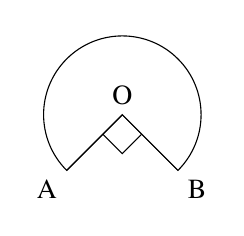
\begin{tikzpicture}[rotate = -45, scale = 1]

  % Define points for the angles
  \coordinate (O) at (0,0);
  \coordinate (A) at (0,-1);
  \coordinate (B) at (1,0);

  % Right angle at B
  \draw pic["$ $", draw=black, angle radius=0.35cm, angle eccentricity=1.5] {right angle = A--O--B};
  
  % Draw the sectors and lines
  \draw (O) -- (A) (O) -- (B);

  % Draw the quadrants
  \draw[fill=white] (O) -- (B) arc [start angle=0, end angle=270, radius=1] -- cycle;
  
  % Label the center
  \node at (O) [above] {O};
  \node at (A) [below left] {A};
  \node at (B) [below right] {B};

\end{tikzpicture}
\end{figure}
\begin{center}
$\text{Figure } 17$
\end{center}
\item Find the area of the shaded region in Figure $18$, if $ABCD$ is a square of side $28\text{ cm}$ and $APD$ and $BPC$ are semicircles.
\begin{figure}[ht]
\centering
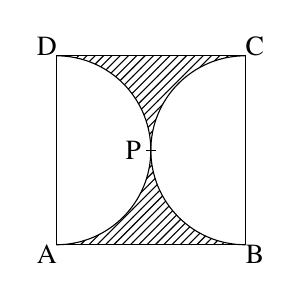
\begin{tikzpicture}[scale=0.6]
  % Draw square
  \draw (0,0) rectangle (4,4);
  
  % Label corners of the square
  \coordinate (O) at (2,4.2);
  \node at (-0.2,-0.2) {A};
  \node at (4.2,-0.2) {B};
  \node at (4.2,4.2) {C};
  \node at (-0.2,4.2) {D};
  \coordinate (P) at (2,2);
  \node at (2,2) [left] {P};
  
  % Draw and fill the area between the arcs
  \begin{scope}
    \clip (0,4) arc[start angle=90, end angle=-90, radius=2] -- 
          (4,0) arc[start angle=-90, end angle=-270, radius=2];
    \fill[pattern=north east lines] (0,0) rectangle (4,4);
  \end{scope}

  % Drawing perpendicular lines
  \draw ($(P)!0.1cm!90:(O)$) -- ($(P)!0.1cm!-90:(O)$);
  
  % Draw arcs again on top of the fill to make them visible
  \draw (0,4) arc[start angle=90, end angle=-90, radius=2];
  \draw (4,0) arc[start angle=-90, end angle=-270, radius=2];

\end{tikzpicture}
\end{figure}
\begin{center}
$\text{Figure } 18$
\end{center}
\item Two tangents $TP$ and $TQ$ are drawn to a circle with centre $O$ from an external point $T$. Prove that $\angle TPQ = 2\angle OPQ$.\\

\item In Figure $19$, $XY$ and $X'Y'$ are two parallel tangents to a circle with centre $O$ and another tangent $AB$ with point of contact $C$ intersects $XY$ at $A$ and $X'Y'$ at $B$. Prove that $\angle AOB = 90\degree$
\begin{figure}[ht]
\centering
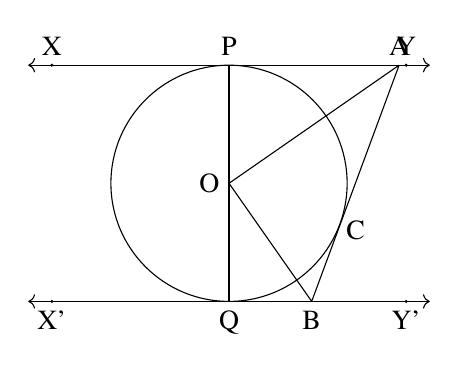
\begin{tikzpicture}[scale = 0.3]

  % Draw the circle
  \draw (0,0) circle (5cm);
  
  % Define points for the angles
  \coordinate (O) at (0,0);
  \coordinate (A) at (7.2,5);
  \coordinate (B) at (3.5,-5);
  \coordinate (C) at (4.55,-2);
  \coordinate (P) at (0,5);
  \coordinate (Q) at (0,-5);
  \coordinate (X) at (-7.5,5);
  \coordinate (Y) at (7.5,5);
  \coordinate (X') at (-7.5,-5);
  \coordinate (Y') at (7.5,-5);

  % Draw the sectors and lines
  \draw (O) -- (A) (O) -- (B) (A) -- (B);
  \draw (P) -- (X) (P) -- (Y) (Q) -- (X') (Q) -- (Y');
  \draw (O) -- (P) (O) -- (Q);

  % Arrows
  \draw[->] (P) -- ($(P)!8.5cm!(X)$);
  \draw[->] (P) -- ($(P)!8.5cm!(Y)$);
  \draw[->] (Q) -- ($(Q)!8.5cm!(X')$);
  \draw[->] (Q) -- ($(Q)!8.5cm!(Y')$);
  
  % Label the center
  \node at (O) [left] {O};
  \node at (A) [above] {A};
  \node at (B) [below] {B};
  \node at (C) [right] {C};
  \node at (P) [above] {P};
  \node at (Q) [below] {Q};
  \node at (X) [above] {X};
  \fill (X) circle (2pt);
  \node at (Y) [above] {Y};
  \fill (Y) circle (2pt);
  \node at (X') [below] {X'};
  \fill (X') circle (2pt);
  \node at (Y') [below] {Y'};
  \fill (Y') circle (2pt);

\end{tikzpicture}
\end{figure}
\begin{center}
$\text{Figure } 19$
\end{center}
\item In Figure $20$, $ABCD$ is a square of side $7\text{ cm}$. $DBPA$ and $DQBC$ are quadrants of circles, each of radius $7\text{ cm}$. Find the area of the shaded region.$\brak{\text{Use } \pi = \frac{22}{7}}$
\begin{figure}[ht]
\centering
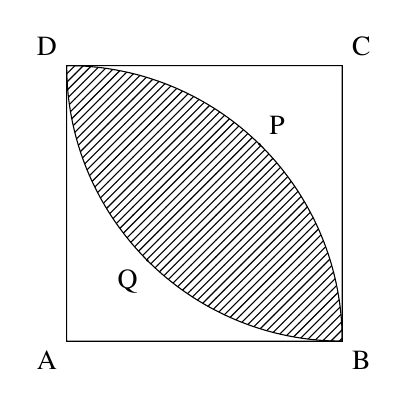
\begin{tikzpicture}[scale=0.5]
    % Draw the square
    \draw (0,0) rectangle (7,7);
    
    % Draw the arcs
    \draw (0,0) -- (7,0) arc [start angle=0, end angle=90, radius=7] -- cycle;
    \draw (7,7) -- (0,7) arc [start angle=180, end angle=270, radius=7] -- cycle;

    % Shade the region between the arcs
    \begin{scope}
        \clip (0,0) -- (7,0) arc [start angle=0, end angle=90, radius=7] -- cycle;
        \fill[pattern=north east lines, pattern color=black] (7,7) -- (0,7) arc [start angle=180, end angle=270, radius=7] -- cycle;
    \end{scope}

    % Label the vertices
    \node at (0,0) [below left] {A};
    \node at (7,0) [below right] {B};
    \node at (7,7) [above right] {C};
    \node at (0,7) [above left] {D};
    \node at (4.9,5) [above right] {P};
    \node at (2.05,2.05) [below left] {Q};
    \fill (4.9,5) circle (1pt);
    \fill (2.05,2.05) circle (1pt);

\end{tikzpicture}
\end{figure}
\begin{center}
$\text{Figure } 20$
\end{center}
\item The length of the minute hand of a clock is $14\text{ cm}$. Find the area swept by the minute hand in $10$ minutes. $\brak{\text{Use } \pi = \frac{22}{7}}$\\
\item Prove that the tangent at any point of a circle is perpendicular to the radius through the point of contact.\\
\end{enumerate}
\section{Probability}
\begin{enumerate}
\item Cards bearing numbers $2, 3, 4, \ldots, 11$ are kept in a bag. A card is drawn at random from the bag. The probability of getting a card with a prime number is\\
\begin{enumerate}
\item $\frac{1}{2}$\\
\item $\frac{2}{5}$\\
\item $\frac{3}{10}$\\
\item $\frac{5}{9}$\\
\end{enumerate}
\item Two dices are thrown together. The probability of getting the same number on both dices is :\\
\begin{enumerate}
\item $\frac{1}{2}$\\
\item $\frac{1}{3}$\\
\item $\frac{1}{6}$\\
\item $\frac{1}{12}$\\
\end{enumerate}
\item The probability of a non-leap year having $53$ Mondays is \\
\begin{enumerate}
\item $\frac{2}{7}$\\
\item $\frac{1}{7}$\\
\item $\frac{5}{7}$\\
\item $\frac{6}{7}$\\
\end{enumerate}
%Probability
\item A card is drawn at random from a well shuffled pack of $52$ cards. Find the probability of getting\\
\begin{enumerate}[label=\Roman*.]
\item a red king.\\
\item a queen or a jack.\\
\end{enumerate}
%Probability
\item All kings, queens and aces are removed from a pack of $52$ cards. The remaining cards are well shuffled and then a card is drawn from it. Find the probability that the drawn card is \\
\begin{enumerate}[label=\Roman*.]
\item a black face card.\\
\item a red card.\\
\end{enumerate}
%probability

%probability
\item A number is selected at random from first $50$ natural numbers. Find the probability that it is a multiple of $3$ and $4$.\\
%probability
\item A box contains $100$ red cards, $200$ yellow cards and $50$ blue cards. If a card is drawn at random from the box, then find the probability that it will be \begin{enumerate}[label=\Roman*.]
\item a blue card
\item not a yellow card
\item neither a yellow nor a blue card.\\
\end{enumerate}

\item A child has a die whose six faces show the letters as given below.The die is thrown once. Find the probability of getting\\
\begin{figure}[ht]
\centering
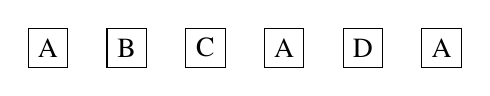
\begin{tikzpicture}[scale = 5]

  % Draw square
  \draw (0,0) rectangle (0.1,0.1);
  \draw (0.2,0) rectangle (0.3,0.1);
  \draw (0.4,0) rectangle (0.5,0.1);
  \draw (0.6,0) rectangle (0.7,0.1);
  \draw (0.8,0) rectangle (0.9,0.1);
  \draw (1,0) rectangle (1.1,0.1);
  
  % Label the center
  \node at (0.05,0.05) {A};
  \node at (0.25,0.05) {B};
  \node at (0.45,0.05) {C};
  \node at (0.65,0.05) {A};
  \node at (0.85,0.05) {D};
  \node at (1.05,0.05) {A};

\end{tikzpicture}
\end{figure}
\begin{enumerate}[label=\Roman*.]
\item A\\
\item D\\
\end{enumerate}
\item Cards marked with numbers $1,3,5, \ldots, 101$ are placed in a bag and mixed thoroughly. A card is then drawn at random from the bag. Find the probability that the number on the drawn card is 
\begin{enumerate}[label=\Roman*.]
\item less than $19$.
\item a prime number less than $20$.\\
\end{enumerate}
\end{enumerate}
\section{Construction}
\begin{enumerate}
\item Draw a triangle $ABC$ with $BC = 7 \text{ cm}$, $\angle B = 45 \degree$ and $\angle C = 60 \degree$. Then construct another triangle, whose sides are $\frac{3}{5}$ times the corresponding sides of $\triangle ABC$.\\
%construction
\item Construct a right triangle in which the sides , (other than the hypotenuse) are of length $6\text{ cm}$ and $8\text{ cm}$. Then construct another triangle, whose sides are $\frac{3}{5}$ times the corresponding sides of the given triangle.\\
\item Draw a right triangle in which the sides (other than the hypotenuse) are of lengths $6\text{ cm}$ and $8\text{ cm}$. then construct another triangle whose sides are $\frac{3}{5}$ times the corresponding sides of the given triangle.\\
\end{enumerate}
\section{Algebra}
\begin{enumerate}
\item The roots of the quadratic equation  $2x^2 - x - 6 = 0$ are\\
\begin{enumerate}
\item $-2,\dfrac{3}{2}$\\
\item $2,-\dfrac{3}{2}$\\
\item $-2,-\dfrac{3}{2}$\\
\item $2,\dfrac{3}{2}$\\
\end{enumerate}
\item If $1$ is a root of the equations $ay^2 + ay + 3 = 0$ and $y^2 + y + b = 0$, then $ab$ equals :\\
\begin{enumerate}
\item $3$\\
\item $-\dfrac{7}{2}$\\
\item $6$\\
\item $-3$\\
\end{enumerate}
\item If the quadratic equation $mx^2 + 2x + m = 0$ has two equal roots, then the values of $m$ are :\\
\begin{enumerate}
\item $\pm 1$\\
\item $0,2$\\
\item $0,1$\\
\item $-1,0$\\
\end{enumerate}
%algebra
\item Find the value of $p$ for which the roots of the equation $px\brak{x-2} + 6 = 0$, are equal.\\
%Algebra
\item Solve the following quadratic equation for $x$ :\\
\begin{align}
x^2 - 4 a x - b^2 + 4a^2 = 0\\
\end{align}
%algebra
%algebra
\item Find the value$\brak{\text{s}}$ of $k$ so that the quadratic equation $x^2 - 4kx + k = 0$ has equal roots.\\
%algebra
\item Solve for $x$: $4x^2 - 4ax + \brak{a^2 - b^2} = 0$\\
%algebra
\item Solve for $x$: $3x^2 - 2\sqrt 6 x + 2 = 0$\\

\item Find the value of $k$ for which the roots of the quadratic equation $\brak{k - 4} x^2 + 2\brak{k-4} x + 2 =0$ are equal.\\
\item Solve for x:\\
$4\sqrt 3 x^2 + 5x - 2\sqrt 3 = 0$\\
\end{enumerate}
\section{Geometry}
\begin{enumerate}
\item A solid right circular cone is cut into two parts at the middle of its height by a plane parallel to its base. The ratio of the volume of the smaller cone to the whole cone is\\
\begin{enumerate}
\item $1 : 2$\\
\item $1 : 4$\\
\item $1 : 6$\\
\item $1 : 8$\\
\end{enumerate}
\item If the radius of the base of a right circular cylinder is halved, keeping the height the same, then the ratio of the volume of the cylinder thus obtained to the volume of original cylinder is :\\
\begin{enumerate}
\item $1 : 2$\\
\item $1 : 4$\\
\item $2 : 1$\\
\item $4 : 1$\\
\end{enumerate}
\item The radii of a circular ends of a bucket of height $40\text{ cm}$ are $24\text{ cm}$ and $15\text{ cm}$. The slant height $\brak{\text{in cm}}$ of the bucket is\\
\begin{enumerate}
\item $51$\\
\item $49$\\
\item $43$\\
\item $41$\\
\end{enumerate}

\item A solid sphere of radius $10.5 \text{ cm}$ is melted and recast into smaller solid cones, each of radius $3.5 \text{ cm}$ and height $3 \text{ cm}$. Find the number of cones so formed. $\brak{\text{Use } \pi = \frac{22}{7}}$\\

\item A hemispherical bowl of internal radius $9 \text{ cm}$ is full of water. Its contents are emptied in a cylindrical vessel of internal radius $6 \text{ cm}$. Find the height of water in the cylindrical vessel.\\


\item A hemispherical tank, full of water, is emptied by a pipe at the rate of $\frac{22}{7}$ litres per sec. How much time will it take to empty half the tank if the diameter of the base of the tank is $3 \text{ m}$?\\

\item A drinking glass in the shape of the frustum of a cone of height $14 \text{ cm}$. The diameters of the two circular ends are $4 \text{ cm}$ and $2 \text{ cm}$. Find the capacity of the glass.  $\brak{\text{Use } \pi = 3.14}$\\

\item  A military tent of height $8.25 \text{ m}$ is in the form of a right circular cylinder of base diameter $30 \text{ m}$ and height $5.5 \text{ m}$ surmounted by a right circular cone of same base radius. Find the length of the canvas use in making tent, if the breadth of the canvas is $1.5 \text{ m}$.\\

\item The volume of a hemisphere is $2425\dfrac{1}{2}$ $\text{ cm}^3$. Find the curved surface area.  $\brak{\text{Use } \pi = 3.14}$\\

\item From a solid cylinder of height $7\text{ cm}$ and base diameter $12\text{ cm}$, a conical cavity of same height and same base diameter is hollowed out. Find the total surface area of the remaining solid. $\brak{\text{Use } \pi = \frac{22}{7}}$\\

\item A cylindrical bucket, $32 \text{ cm}$ high and with radius of base is $18 \text{ cm}$, is filled with sand. This bucket is emptied on the ground and a conical heap of sand is formed. If the height of the conical heap is $24 \text{ cm}$, then find the radius sand slant height of the heap.\\


\item A solid is in the shape of a cone surmounted on a hemisphere, the radius of each of them being $3.5\text{ cm}$ and the total height of solid is $9.5\text{ cm}$. Find the volume of the solid. $\brak{\text{Use } \pi = \frac{22}{7}}$\\

\item A bucket is in the form of a frustum of a cone and it can hold $28.499$ litres of water. If the radii of its circular ends are $28\text{ cm}$ and $21\text{ cm}$, find the height of the bucket. $\brak{\text{Use } \pi = \frac{22}{7}}$\\


\item A solid is in the shape of a cone mounted on a hemisphere of same base radius. If the curved surface area of the hemispherical part and the conical part are equal, then find the ratio of the radius and the height of the conical part.\\

\item A sphere of diameter $6\text{ cm}$ is dropped into a cylindrical vessel, partly filled with water, whose diameter is $12\text{ cm}$. If the sphere is completely submerged in water, by how much will the surface of water be raised in cylindrical vessel ?\\
\item A toy is in the shape of a cone mounted on a hemisphere of same base radius. If the volume of the toy is $231\text{ cm}^3$ and its diameter is $7\text{ cm}$, then find the height of the toy.  $\brak{\text{Use } \pi = \frac{22}{7}}$\\

\item The radii of internal and external surfaces of a hollow spherical shell are $3\text{ cm}$ and $5\text{ cm}$ respectively. It is melted and recast into a solid cylinder of diameter $14\text{ cm}$. Find the height of the cylinder.\\

\item A drinking glass is in the shape of a frustum of a cone of height $14\text{ cm}$. The diameters of its two circular ends are $16\text{ cm}$ and $12\text{ cm}$. Find the capacity of the glass. $\brak{\text{Use } \pi = \frac{22}{7}}$\\

\end{enumerate}
\section{Discrete}
\begin{enumerate}
\item If the $n^{th}$ term of an $A.P$ is $\brak{2n+1}$, then sum of its first three terms is\\
\begin{enumerate}
\item $6n + 3$\\
\item $15$\\
\item $12$\\
\item $21$\\
\end{enumerate}
\item The next terms of $A.P.$ $\sqrt {18}, \sqrt {50}, \sqrt {98}, \ldots$ is\\
\begin{enumerate}
\item $\sqrt {146}$\\
\item $\sqrt {128}$\\
\item $\sqrt {162}$\\
\item $\sqrt {200}$\\
\end{enumerate}
%discrete
\item Find the common difference of an $A.P$ whose first term is $5$ and the sum of its first four terms is half the sum of the next four terms.\\
%discrete
\item The $17th$ term of an $AP$ is $5$ more than twice its $8th$ term. If the $11th$ term of the $AP$ is $43$, then find the $nth$ term.\\

\item Sum of the first $14$ terms of an $AP$ is $1505$ and its first term is $10$. find its $25th$ term.\\
\item In an $A.P.$, the first term is $12$ and the common difference is $6$. If the last term of the $A.P.$ is $252$, find its middle term.\\
\item If $4$ times the fourth term of an $A.P.$ is equal to $18$ times its $18^{th}$ term, then find its $22^{th}$ term.\\
\item The sum of $4^{th}$ and $8^{th}$ term terms of an $A.P.$ is $24$ and the sum of its $6^{th}$ and $10^{th}$ terms is $44$. Find the sum of first ten terms of the $A.P.$\\
\end{enumerate}
\section{Number Systems}
\begin{enumerate}
\item The sum of first 20 odd natural numbers is :\\
\begin{enumerate}
\item $100$\\
\item $210$\\
\item $400$\\
\item $420$\\
\end{enumerate}
\item How many two-digit numbers are divisible by 3?\\
%Number systems
\item If the sum of two natural numbers is $8$ and their product is $15$, find the numbers.\\
%Number systems
\item Find the sum of all multiples of 7 lying between $500$ and $900$.\\
%NUmber systems
\item The number of a fraction is $3$ less than its denominator. If $1$ is added to the denominator, the fraction is decreased by $\frac{1}{15}$. Find the fraction.\\
%number systems

%number systems
\item Find the sum of all three digit natural numbers, which are multiples of $11$.\\
\item A shopkeeper buys some books for $\textcurrency 80$. If he had bought $4$ more books for the same amount, each book would have to cost $\textcurrency 1$ less. Find the number of books he bought.\\

\item The sum of two numbers is $9$ and the sum of their reciprocals is $\dfrac{1}{2}$. Find the numbers.\\
\item Find the sum of first 40 positive integers divisible by $6$.\\
\item A two-digit number is such that the product of its digits is $14$. When $45$ is added to the number, the digits interchange their places. Find the number.\\
\item Find two consecutive natural numbers, the sum of whose squares is $145$.\\
\end{enumerate}
\section{Trigonometry}
\begin{enumerate}
\item A kite is flying at a height of $30 \text{ m}$ from the ground. The length of string from the kite to the ground is $60 \text{ m}$. Assuming that there is no slack in the string, the angle of elevation of the kite at the ground is\\
\begin{enumerate}
\item $45\degree$\\
\item $30\degree$\\
\item $60\degree$\\
\item $90\degree$\\
\end{enumerate}
\item From a point on the ground, which is $15\text{ m}$ away from the foot of a vertical tower, the angle of elevation of the top of the tower, is found to be $60\degree$. The height of the tower in $\brak{\text{in metres}}$ is\\
\begin{enumerate}
\item $5\sqrt 3$\\
\item $15\sqrt 3$\\
\item $15$\\
\item $7.5$\\
\end{enumerate}
\item The length of shadow of a tower on the plane ground is $\sqrt 3 \text{ m}$ times the height of the tower. The angle of elevation of sun is :\\
\begin{enumerate}
\item $45\degree$\\
\item $30\degree$\\
\item $60\degree$\\
\item $90\degree$\\
\end{enumerate}
%Trigonometry
\item The angles of depression of the top and bottom of a tower as seen from the top of a $60\sqrt 3 \text{ m}$ high cliff are $45\degree$ and $60\degree$ respectively. Find the height of the tower.\\
%Trigonometry
\item In a flight of $2800 \text{ km}$, an aircraft was slowed down due to bad weather. Its average speed is reduced by $100 \text{ km/h}$ and time is increased by $30$ minutes. Find the original duration of flight.\\
%Trigonometry
\item The angles of elevation and depression of the top and bottom of a light-house from the top of a $60 \text{ m}$ high building are $30\degree$ and $60\degree$ respectively. Find\\
\begin{enumerate}[label=\Roman*.]
\item the difference between the heights of the light-house and the building.\\
\item the distance between light-house and building.\\
\end{enumerate}
%trigonometry
\item The angles of depression of two ships from the top of a light house and on the same side of it are found to be $45\degree$ and $30\degree$. if the ships are $200 \text{ km}$ apart, find the height of the light house.\\
\item The angle of elevation of the top of a hill at the foot of a tower is $60\degree$ and the angle of depression from the top of the tower of the foot of the hill is $30\degree$. If the tower is $50\text{ m}$ high, find the height of the hill.\\
\item From the top of a tower $50\text{ m}$ high, the angle of depression of the top of a pole is $45\degree$ and from the foot of the pole, the angle of elevation of the top of the tower is $60\degree$. find the height of the pole if the pole and tower stand on the same plane.\\
\item The angle of depression from the top of a tower of a point $A$ on the ground is $30\degree$. On moving a distance of $20\text{ m}$ from the point $A$ towards the foot of the tower to a point $B$ the angle of elevation of the top of the tower from point $B$ is $60\degree$. Find the height of the tower and its distance from point $A$.
\end{enumerate}
\end{document}
